\documentclass[]{beamer}

%%%%%%%%%%%%%%%%%%%%%%%%%%%%%%%%%%%%%%%%%%%%%%%%%%%%%%%%%%
% Slides pour la présentation de Rathaxes interne au LSE %
%%%%%%%%%%%%%%%%%%%%%%%%%%%%%%%%%%%%%%%%%%%%%%%%%%%%%%%%%%

\usepackage[francais]{babel}
\usepackage{rtxslides}

\title{\rtx}
\subtitle{Un DSL et son compilateur}
\author{David Pineau \\ \texttt{<david@lse.epitech.eu>}}

\begin{document}

\begin{frame}
\titlepage
\end{frame}



\section{Présentation du projet}

\subsection{Le projet}
\begin{frame}
\frametitle{Qu'est-ce que c'est}
\rtx\ est un compilateur et un langage dédié. L'objectif est de permettre la
génération du code C d'un pilote de périphérique à partir d'une description
algorithmique du périphérique. Le compilateur peut générer le code du pilote de
périphérique en C pour n'importe quel système d'exploitation supporté.
\end{frame}

\subsection{Problématique}
\begin{frame}
\frametitle{Problématique du développement de pilote}
\begin{enumerate}[<+->]
    \item Multiples compétences :
        \begin{itemize}[<1->]
            \item Électronique : compréhension du matériel ;
            \item Développement noyau : connaissance de l'OS cible.
        \end{itemize}
    \item Code critique ;
    \item Longue auto formation.
\end{enumerate}
\end{frame}

\subsection{Solution}
\begin{frame}
\frametitle{Les solutions}
\begin{itemize}[<+->]
    \item Séparation des compétences ;
    \item Vérifications multiples.
\end{itemize}
\end{frame}



\section{Définir un langage dédié}

\subsection{Les besoins du langage}
\begin{frame}
\frametitle{Ce qui est nécessaire}
\begin{itemize}[<+->]
    \item Souplesse, évolutivité ;
    \item Redondance ;
    \item Réunir les différentes compétences.
\end{itemize}
\end{frame}

\subsection{Les trois points focaux}
\begin{frame}
\frametitle{Un DSL en trois parties}
% The parameter must be either :
% - 't' for top alignment;
% - 'c' for center alignment;
% - 'b' for bottom alignment.
\begin{columns}[c]
% Maximum 3 columns : l for left, c for center, r for right
    % Left column for Front-end (Electronician)
    \begin{column}[l,T]{115pt}
        \uncover<2-> {
            \begin{center} \large{\itshape{Développeur Driver}} \end{center}
            \begin{center}
                \setlength\fboxsep{0.5pt}
                \setlength\fboxrule{0.5pt}
                %\fbox{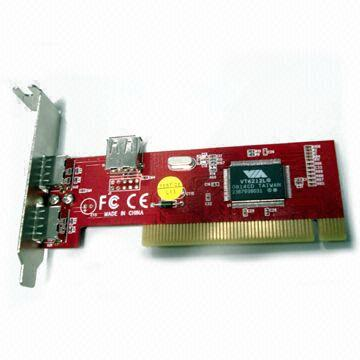
\includegraphics[height=70pt]{pictures/pci_card.jpg}}
                \fbox{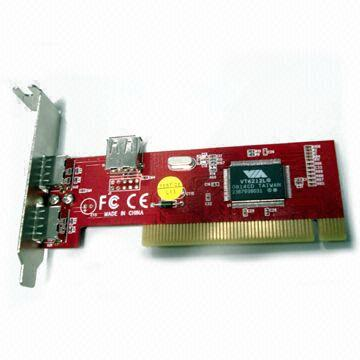
\includegraphics[scale=0.2]{pictures/pci_card.jpg}}
            \end{center}
            \scriptsize{
                Description du périphérique :
                \begin{itemize}
                    \item Registres ;
                    \item Algorithmes.
                \end{itemize}
            }
        }
    \end{column}

    % Center column for Middle-end (\rtx\ Maintainer)
    \begin{column}[c,T]{115pt}
        \uncover<3-> {
            \begin{center} \large{\itshape{Développeur \rtx}} \end{center}
            \scriptsize{
                Identification des sémantiques communes à tous les systèmes
                d'exploitation afin d'en tirer un modèle générique.
            }
        }
    \end{column}
    
    % Right column for Back-end (OS developer)
    \begin{column}[r,T]{115pt}
        \uncover<4-> {
            \begin{center} \large{\itshape{Développeur Système}} \end{center}
            \scriptsize{
                Code spécifique aux systèmes d'exploitation. Requiert des
                connaissances systèmes poussées.
            }
        }
    \end{column}

    \transdissolve<2>
    \transdissolve<3>
    \transdissolve<4>
\end{columns}
\end{frame}

\subsection{Le rôle de chaque partie du DSL}
\begin{frame}
\frametitle{Un DSL en trois parties}
\begin{columns}[c]
    
    \begin{column}[l,T]{115pt}
        \begin{center} \large{\itshape{Front-End}} \end{center}
        \scriptsize{
            \begin{center} Fichier \texttt{.rtx} \end{center}
            Il permet de décrire :
            \begin{itemize}
                \item un périphérique (registres) ;
                \item les sous-systèmes qu'il utilise (PCI, I2C, etc\ldots) ;
                \item les algorithmes que le pilote doit implanter.
            \end{itemize}
        }
    \end{column}
    
    \begin{column}[c,T]{115pt}
        \begin{center} \large{\itshape{Middle-End}} \end{center}
        \scriptsize{
            \begin{center} Fichier \texttt{.rti} \end{center}
            Il contient des interfaces décrivant :
            \begin{itemize}
                \item Des Types ;
                \item Des Séquences ;
                \item Des variables de configuration.
            \end{itemize}
        }
    \end{column}
    
    \begin{column}[r,T]{115pt}
        \begin{center} \large{\itshape{Back-End}} \end{center}
        \scriptsize{
            \begin{center} Fichier \texttt{.blt} \end{center}
            Il permet d'implémenter le code système-spécifique correspondant
            aux interfaces associées. On y retrouvera :
            \begin{itemize}
                \item Des templates de type ;
                \item Des templates de séquence.
            \end{itemize}
        }
    \end{column}

\end{columns}
\transdissolve<1>
\end{frame}

\subsection{Ce que cela implique pour le compilateur}
\begin{frame}
\end{frame}



\section{Un compilateur hors normes}

\subsection{Compilateur ``coordonné''}
\begin{frame}
\end{frame}

\subsection{Compilateur ``non coordonné''}
\begin{frame}
\end{frame}



\end{document}
